\section{AlphaZero-like Self-Play: A Renewable Verifiable Reward Source}

We now specialize the traditional \rl{} comparison to AlphaZero-like self-play in board games. This is the cleanest contrast to fixed-dataset \llm{} \rlvr{}: both settings may use terminal, sparse, verifiable rewards, but AlphaZero-like training continually generates new games against a policy of comparable strength. As a result, the terminal reward distribution can remain high-variance throughout training, rather than collapsing as the model solves or fails a fixed set of prompts.

\subsection{Self-Play Keeps the Outcome Near the Decision Boundary}

Consider a two-player zero-sum game. At training time $t$, an AlphaZero-like agent uses the current policy/value model, often combined with Monte Carlo tree search, to generate self-play games. A trajectory
\[
  \tau \sim q_{\theta(t),\theta(t)}(\cdot)
\]
is produced by matching the current agent against itself. The terminal reward from one player's perspective is
\[
  z(\tau)\in\{0,1\},
\]
where $1$ denotes a win and $0$ denotes a loss. Draws can be ignored, folded into a half reward, or handled as a third outcome; the binary case makes the information argument most transparent.

The local reward-side signal is
\[
  \mathcal{V}_{\theta(t)}^{\mathrm{sp}}
  =
  \Var_{\tau\sim q_{\theta(t),\theta(t)}}[z(\tau)]
  =
  p_t(1-p_t),
\]
where
\[
  p_t=\Pr_{\tau\sim q_{\theta(t),\theta(t)}}[z(\tau)=1].
\]
Because the two players are copies of the same learning system, self-play tends to keep the matchup balanced. Up to first-move advantage, stochasticity, search noise, and draw handling, one should expect
\[
  p_t \approx \frac{1}{2},
  \qquad
  \mathcal{V}_{\theta(t)}^{\mathrm{sp}}
  \approx
  \frac{1}{4}.
\]
Thus the reward distribution remains approximately ``half zero, half one.'' Unlike a fixed prompt whose verifier outcomes may become all-correct or all-wrong, a self-play game does not become trivial merely because the agent improves: its opponent improves with it.

\subsection{The Information Integral Need Not Saturate}

Using the global reward-information definition from Section~2, the self-play reward-information mass is
\[
  \mathcal{I}_{\mathrm{sp}}(T)
  =
  \int_0^T
  \alpha(t)
  \Var_{\tau\sim q_{\theta(t),\theta(t)}}[z(\tau)]
  dt.
\]
If self-play keeps the terminal outcome non-degenerate, i.e. there exists a constant $c>0$ such that
\[
  \Var_{\tau\sim q_{\theta(t),\theta(t)}}[z(\tau)]\ge c
  \quad
  \text{for most }t,
\]
then
\[
  \mathcal{I}_{\mathrm{sp}}(T)
  \ge
  c\int_0^T \alpha(t)\,dt.
\]
Therefore, whenever the cumulative update budget $\int_0^T\alpha(t)dt$ grows without bound, the self-play information integral is also unbounded. Even for finite training, the key point is that the information budget is controlled by the number of generated self-play games and the cumulative update mass, not by a fixed dataset size.

This is the fundamental difference from fixed-dataset \llm{} \rlvr{}. For a fixed prompt set with deterministic binary verifiers, each prompt has a bounded reward-variance mass and the dataset total is bounded by a quantity scaling with $N$. In AlphaZero-like self-play, there is no fixed list of questions whose outcomes are gradually exhausted. The learner keeps producing fresh games against its current level, and the terminal reward remains a renewable source of high-variance feedback.

\subsection{Why Improvement Does Not Collapse Reward Variance}

The apparent paradox is that the agent becomes stronger, yet its win-rate in self-play does not approach one. The reason is that self-play measures the current policy against a moving reference. Let $\pi_{\theta(t)}$ be the current policy and suppose both sides use the same or closely related policy. Then absolute playing strength can improve while the self-play win probability remains close to balanced:
\[
  \Pr(\pi_{\theta(t)} \text{ beats } \pi_{\theta(t)}) \approx \frac{1}{2}.
\]
This makes self-play an automatic curriculum. The task distribution tracks the learner's ability: when the model improves, the opponent and generated positions improve as well. The verifier still gives only a terminal outcome, but the rollout distribution continually refreshes the set of contested decisions that can affect the outcome.

From the covariance view, this means AlphaZero-like training attempts to maintain nonzero covariance between terminal outcome and policy-score directions:
\[
  g_{\mathrm{sp}}(\theta)
  =
  \Cov_{\tau\sim q_{\theta,\theta}}
  \left(
    z(\tau),
    \nabla_\theta \log q_\theta(\tau)
  \right).
\]
The terminal reward is sparse, but it is repeatedly queried at the frontier of the current policy's competence. This is exactly the regime where $p(1-p)$ is large.

\subsection{Connect Four Evidence}

We tested this distinction in two rounds of Connect Four experiments. The results support the view that AlphaZero-like self-play is fundamentally different from fixed-dataset \rlvr{}. With a fixed prompt or verifier source, improvement eventually pushes many examples into all-correct or all-wrong regimes, where the binary verifier carries little local contrast. In self-play, by contrast, the opponent and the position distribution co-evolve with the current policy. The training data therefore keeps moving toward the model's competence boundary. Even though the reward remains only a terminal $0/1$ outcome, self-play can sustain substantial outcome variance and act as a renewable source of verifier feedback.

\begin{figure}[t]
  \centering
  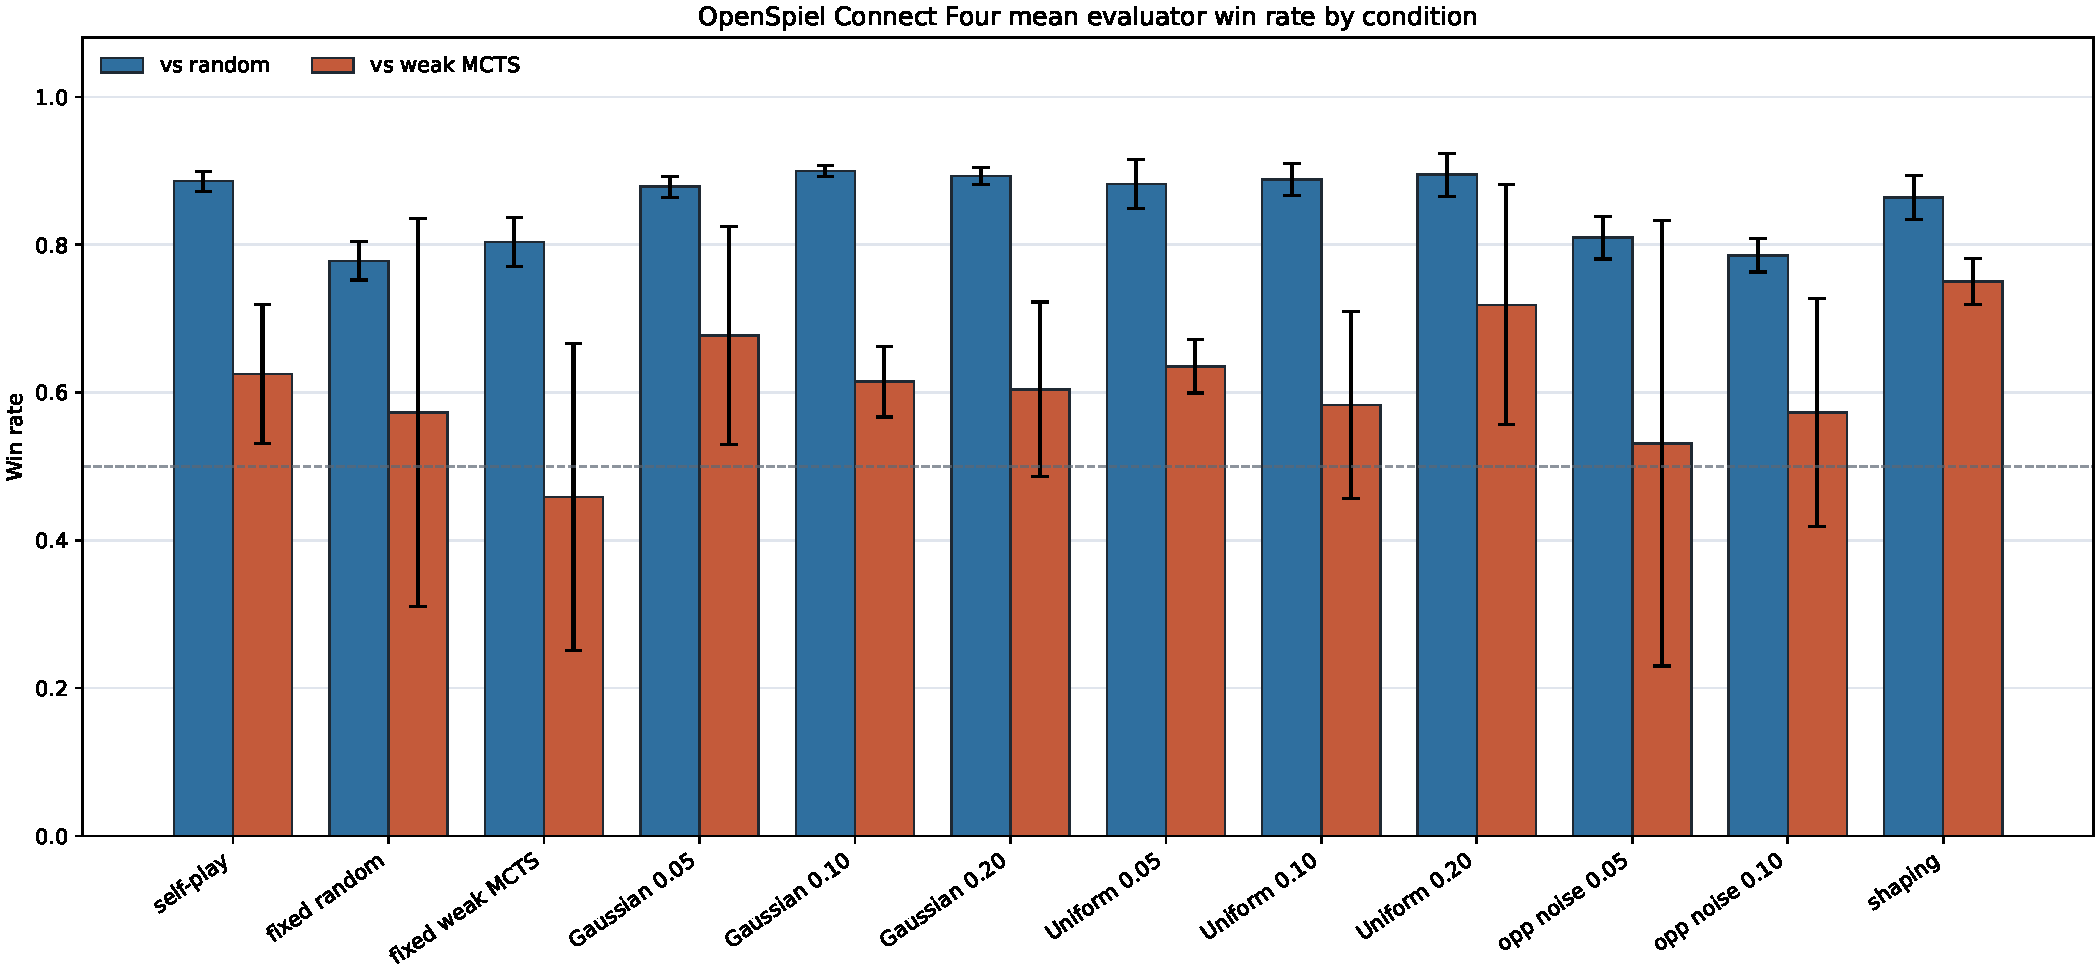
\includegraphics[width=0.86\linewidth]{figures/openspiel_c4_mean_win_rate_by_condition.pdf}
  \caption{Connect Four evaluation under different training conditions. Self-play renews the opponent and state distribution as the policy changes, whereas fixed or noisy sources can increase update magnitude without necessarily improving external performance.}
  \label{fig:connect-four-self-play}
\end{figure}

The experiments also show why reward variance, outcome entropy, or parameter-update norm should not be identified directly with usable information. Fixed opponents and noisy opponent actions can produce larger gradient norms and parameter updates, but this does not by itself improve external evaluation. Larger updates may reflect distributional instability or target drift rather than stronger learning. Reward-noise results point in the same direction: small or moderate terminal noise can be tolerable in the OpenSpiel setting and may even have a mild regularizing effect, while higher noise in a separate value-fitting experiment clearly degrades learning. Noise variance itself is therefore not information. Only reward variation aligned with policy-controllable differences among trajectories can become an effective training signal.

\subsection{Implications for the RLVR Bottleneck}

AlphaZero-like self-play suggests a useful baseline for thinking about information bottlenecks:
\begin{enumerate}
  \item \textbf{The verifier can be terminal and binary.} The reward channel is still low-bandwidth at the trajectory level.
  \item \textbf{The rollout distribution is adaptive.} Self-play keeps generating trajectories near the current decision boundary.
  \item \textbf{The reward variance need not decay.} Because the opponent is the current policy, the outcome distribution remains close to balanced.
  \item \textbf{The global information integral can keep growing.} With continuing self-play and non-vanishing cumulative update budget, the total reward-information mass is not capped by a fixed dataset.
\end{enumerate}

This explains why AlphaZero-like methods can learn from terminal verifiable rewards despite their local low bandwidth. They do not solve the bottleneck by making each reward more informative; they solve it by making the feedback source renewable and by keeping the model near a high-variance self-play frontier. Fixed-dataset \llm{} \rlvr{} lacks this mechanism by default, which is why its information budget is much more likely to saturate.
